\subsection{Experimentos}

En los experimentos siguiente fijaremos el quantum en un ciclo de reloj, el costo de cambio de contexto también en un ciclo y el costo de migrar entre núcleos en dos ciclos de reloj.

\subsubsection{Primer experimento:} 

En este primer experimento utilizaremos un lote de tres procesos que utilizan intensivamente el CPU:
\begin{quote}
@1\\
TaskCPU 5\\
@3\\
TaskCPU 4\\
@4\\
TaskCPU 4\\
\end{quote}

Solo utilizamos un núcleo de procesamiento, ya que lo que nos interesa mostrar en este experimento es que los procesos se ejecutan de la forma en que Round Robin lo especifica. A continuación el gráfico resultante:

\begin{figure}[H]
\begin{center}
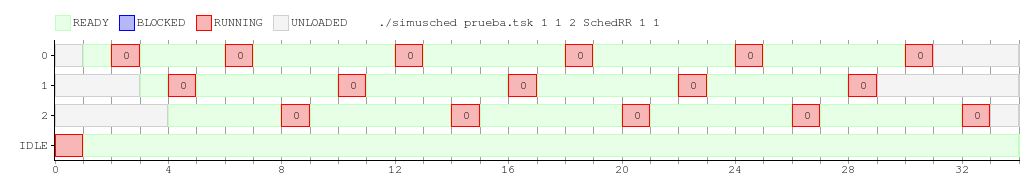
\includegraphics[width=1.1\textwidth]{img/salida_ej4_1.png}
     \caption{Experimentación de Round Robin}
\end{center}
\end{figure}

\textbf{Conclusiones:}

Los procesos se ejecutan de forma alternada, a medida que se van agregando a la lista de procesos \textit{ready}, y solo durante el quantum especificado.

\subsubsection{Segundo experimento:} 

En este segundo experimento utilizamos un lote con seis procesos. Tres procesos que utilizan intensivamente el CPU y tres procesos que realizan operaciones de E/S. El lote utilizado es el siguiente:

\begin{quote}
@1\\
TaskCPU 5\\
@2\\
TaskConsola 3 3 3\\
@3\\
TaskCPU 4\\
@4\\
TaskCPU 4\\
TaskConsola 2 4 4\\
@5\\
TaskConsola 1 5 5\\
\end{quote}

Fijamos en dos (2) la cantidad de núcleos del procesador, ya que con un solo núcleo no es posible observar que el scheduler realmente realiza migraciones de procesos entre núcleos, y con mas de dos núcleos no se obtiene ninguna información del scheduler que no se obtenga con dos núcleos.

A continuación, el gráfico resultante de ejecutar el lote de procesos con el scheduler Round-Robin:

\begin{figure}[H]
\begin{center}
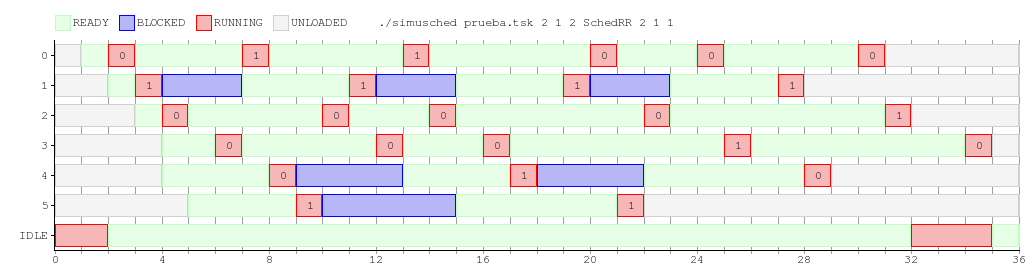
\includegraphics[width=1.1\textwidth]{img/salida_ej4_2.png}
     \caption{Experimentación de Round Robin}
\end{center}
\end{figure}

\textbf{Conclusiones:} 

Como se puede ver en el gráfico, los procesos se ejecutan en el primer núcleo que este libre independientemente de si se ejecuto previamente en ese núcleo o no, permitiendo así la migración de procesos entre núcleos.
También se puede ver que los procesos solo se ejecutan durante el quantum especificado y luego son desalojados para permitir a otro proceso utilizar el procesador.
Cuando un proceso se desbloquea o consume todo su quantum es añadido al final de la cola de procesos \textit{ready} lo cual, en muchos casos, altera el orden en el cual se ejecutan los procesos, es decir, los procesos no siempre se ejecutan en el orden en el cual llegaron.











